% Final project report, Springer LNCS format (llncs.cls v2.26).
% Source of every number: reports/project_report.md.
% Build: tectonic main.tex   (or upload this folder to Overleaf)
\documentclass[runningheads]{llncs}

\usepackage[T1]{fontenc}
\usepackage{graphicx}
\usepackage{amsmath,amssymb}
\usepackage{booktabs}
\usepackage{xcolor}
\usepackage{pgfplots}
\pgfplotsset{compat=1.18}
\usepackage{hyperref}
\hypersetup{hidelinks}
\setlength{\tabcolsep}{5pt}

% Chart colours (validated categorical pair)
\definecolor{sF}{HTML}{2A78D6}   % validation F1
\definecolor{sA}{HTML}{EB6834}   % validation ROC-AUC
\definecolor{ink2}{HTML}{55554F}
\definecolor{phasebg}{HTML}{F1F0EC}

% Marks a value taken from a written project report rather than a saved output.
\newcommand{\doc}{$^\dagger$}

\begin{document}

\title{Unsupervised Anomaly Detection in Batch-Distillation Sensor Data: From a Hybrid Baseline to a Mahalanobis-Scored Convolutional Autoencoder}
\titlerunning{Anomaly Detection in Batch-Distillation Sensor Data}

\author{Bhuvana Shikaripura Dasharatha \and Purna Chandra Nandigana}
\authorrunning{B. Shikaripura Dasharatha and P. C. Nandigana}
\institute{RPTU Kaiserslautern-Landau, Master Project: Machine Learning 26\\Group ML\_DL\_5}

\maketitle

\begin{abstract}
We detect anomalous timesteps in 18-sensor recordings of a laboratory batch-distillation process. The 28 training runs carry no labels, 10 validation runs are labelled per timestep, and 53 test runs are scored on an external Codabench portal, so we treat the task as novelty detection. The project ran in two phases. Phase~1 built a correct evaluation pipeline around a hybrid of a convolutional autoencoder and an Isolation Forest, fixed six correctness bugs, and improved the autoencoder with checkpoint selection and a dilated architecture; it ended with a portal F1 of 0.399 (public) / 0.471 (private). Phase~2 replaced the flat reconstruction error with a per-sensor Mahalanobis score and an F$_{0.5}$ threshold, which raised validation ROC-AUC from 0.605 to 0.768. Fusion with a Local Outlier Factor detector was tested under run-grouped cross-validation and rejected, leaving the autoencoder alone. The final submission scored \textbf{F1 = 0.63 on the portal} (validation F1 0.602, ROC-AUC 0.763). Later robustness checks found no further improvement and showed that the validation estimate is optimistic by 0.070 ROC-AUC and 0.058 F1.
\keywords{Anomaly detection \and Multivariate time series \and Convolutional autoencoder \and Mahalanobis distance}
\end{abstract}

%======================================================================
\section{Introduction}
%======================================================================

Industrial processes are monitored by many sensors, and faults often appear as a change in the joint behaviour of several sensors rather than as a single out-of-range value~\cite{malhotra2016lstm,hundman2018detecting,audibert2020usad}. This project detects such changes at the level of individual timesteps for a university competition.

The defining constraint is the label situation: the training runs are unlabelled and only ten validation runs carry labels. A supervised classifier cannot be trained on anomalies, so every detector in this project models normal behaviour and scores departures from it.

The report follows the two phases of the work:
\begin{itemize}
  \item \textbf{Phase 1} (June to 10 July 2026): baselines, a rebuilt and debugged pipeline, and improvements to the autoencoder itself (Section~\ref{sec:phase1}).
  \item \textbf{Phase 2} (10 to 12 July 2026): a new anomaly score, a tested-and-rejected fusion step, and the final model with portal F1 = 0.63 (Section~\ref{sec:phase2}).
\end{itemize}
Section~\ref{sec:robust} reports checks carried out on the final model in September 2026, after the 0.63 submission; they did not change it.

Unless stated otherwise, numbers are \emph{validation} metrics, computed point-wise over the 79{,}688 labelled validation timesteps. \emph{Portal} scores come from the external competition server and are a different quantity. Values marked \doc{} are taken from project reports written at the time; their raw run outputs were not stored. All other values were read from saved output files.

%======================================================================
\section{Data and Task}
%======================================================================

The data come from a laboratory batch-distillation plant with 18 sensors sampled at 1\,Hz: two levels, nine temperatures, two mass flows, one differential pressure, two pressures and one cooling-medium flow. There are no missing values. Table~\ref{tab:data} lists the splits.

\begin{table}[ht]
\centering
\caption{Data splits.}\label{tab:data}
\begin{tabular}{lrrl}
\toprule
Split & Runs & Timesteps & Labels \\
\midrule
Train & 28 & 189{,}444 & none (described by the organizers as normal runs) \\
Validation & 10 & 79{,}688 & per timestep; 19{,}086 anomalous (23.95\%) \\
Test & 53 & 316{,}024 & hidden; scored by the portal \\
\bottomrule
\end{tabular}
\end{table}

The anomaly rate varies strongly between validation runs, from 0.8\% (run~4) to 81.4\% (run~8), and the ten runs contain 28 anomalous segments in total. There is no separate labelled test split: the ten labelled runs serve both for tuning and for every local metric.

For every test timestep the model must output 0 (normal) or 1 (anomalous) in a CSV with columns \texttt{run\_id}, \texttt{timestep}, \texttt{prediction}. The organizer README states that the portal evaluates submissions with binary F1; it does not say whether F1 is computed point-wise, per run or per event.

%======================================================================
\section{Phase 1: Baselines and a Correct Pipeline}\label{sec:phase1}
%======================================================================

\subsection{Exploratory Analysis and Isolation Forest Baseline}

Exploratory analysis grouped the sensors by the shape of their value distributions and filtered them by correlation (threshold 0.85), keeping 16 of 18 sensors (LS701 and LS702 were dropped). This selection is used only by the tabular detectors; the autoencoder uses all 18 sensors.

The first baseline was an Isolation Forest~\cite{liu2008isolation} (300 trees) on 216 tabular features: the 16 selected sensors, five temporal features per sensor (lag, difference, rolling mean, rolling standard deviation, exponentially weighted mean) and 120 pairwise products. With the threshold at the F1-optimal point of the validation precision--recall curve it reached \textbf{F1 = 0.437} and ROC-AUC 0.585, while flagging 67.5\% of validation timesteps against a true rate of 24\%.

\subsection{The Original Hybrid and Six Correctness Bugs}

The first deep model was a hybrid: a shallow 1D convolutional autoencoder (one convolution block, kernel size 3) fused with a window-level Isolation Forest at a fixed weight of 0.85/0.15. Its reported F1 of about 0.62\doc{} was measured on window-level labels and could not be reproduced from any saved output, so we treat it as historical only.

Rebuilding the notebooks into a single pipeline (Round~1) exposed six bugs, all fixed:
\begin{enumerate}
  \item sliding windows crossed the boundaries between runs;
  \item the threshold was taken from the wrong index of the precision--recall curve (off by one);
  \item the Isolation Forest window features were flattened incorrectly;
  \item scoring and evaluation were done per window instead of per timestep;
  \item the training length had reverted from 50 to 10 epochs;
  \item the fusion weight was hand-set instead of chosen on validation.
\end{enumerate}
From this point on every metric is point-wise over timesteps, windows never cross runs, and each timestep receives one score as the mean over all windows that contain it.

\subsection{Improving the Autoencoder}

\paragraph{Round 1: corrected pipeline.} After the fixes, validation F1 was 0.408\doc{} for the autoencoder, 0.491\doc{} for the Isolation Forest and 0.494\doc{} for the fused hybrid. The hybrid submission scored \textbf{0.399 (public) / 0.471 (private)}\doc{} on the portal.

\paragraph{Round 2: checkpoint selection.} Training loss fell steadily for all 50 epochs, but validation F1 did not follow it. We therefore evaluate the model every 5 epochs and keep the checkpoint with the best validation score. Autoencoder F1 rose to 0.458 (ROC-AUC 0.614). A sweep over the Isolation Forest contamination parameter (0.1--0.3) gave identical F1 (0.491\doc) for every value, because the pipeline thresholds the continuous score directly and contamination only moves the library's internal cut-off.

\paragraph{Round 3: dilated architecture.} A window-size sweep on the shallow model (5-epoch runs, window-level labels) had shown F1 rising from 0.409 to 0.470 as the window grew from 50 to 200 timesteps, which suggested that anomalies develop slowly and need wide context. We replaced the shallow encoder with stacked dilated residual blocks (dilations 1, 2, 4, 8)~\cite{bai2018empirical,oord2016wavenet}. Autoencoder F1 rose to 0.484\doc, but ROC-AUC did not improve (0.605\doc) and the F1-optimal threshold flagged 89.4\%\doc{} of validation timesteps.

\subsection{Where Phase 1 Ended}

Table~\ref{tab:phase1} summarises Phase~1. Two problems remained. First, ranking quality was low: ROC-AUC stayed around 0.6 through all three rounds, so the gains in F1 came mostly from where the threshold was placed. Second, the F1-optimal threshold flagged far more timesteps than are anomalous. The hybrid's F1 stayed at 0.494 throughout, limited by the Isolation Forest rather than the autoencoder.

\begin{table}[ht]
\centering
\caption{Phase 1 results (validation; the portal score is in the last row).}\label{tab:phase1}
\begin{tabular}{llccc}
\toprule
Stage & Change & CNN F1 & CNN ROC-AUC & Hybrid F1 \\
\midrule
Baseline & Isolation Forest (IF) & \multicolumn{2}{c}{IF: 0.437 / 0.585} & -- \\
Round 1 & rebuilt pipeline, 6 bug fixes & 0.408\doc & 0.574\doc & 0.494\doc \\
Round 2 & checkpoint selection & 0.458 & 0.614 & 0.494 \\
Round 3 & dilated residual architecture & 0.484\doc & 0.605\doc & 0.494\doc \\
\midrule
\multicolumn{5}{l}{Portal F1 of the Phase 1 hybrid: 0.399 (public) / 0.471 (private)\doc} \\
\bottomrule
\end{tabular}
\end{table}

%======================================================================
\section{Phase 2: Final Method and Result}\label{sec:phase2}
%======================================================================

Phase~2 kept the dilated architecture from Round~3 and changed how its output is turned into an anomaly score and a decision. The full pipeline is: standard scaling fitted on the training runs, per-run windows of $200 \times 18$, the dilated autoencoder, per-sensor reconstruction error, a Mahalanobis score, averaging to one score per timestep, and a single global threshold.

\subsection{Model and Training}

Table~\ref{tab:arch} gives the architecture. Each residual block consists of two convolutions (kernel size 3, dilation $d$, symmetric padding) with batch normalisation and ReLU, plus a shortcut ($1\times1$ convolution when the channel count changes). The encoder's receptive field is $1 + 4(1+2+4+8) = 61$ timesteps, and the model has 59{,}858 trainable parameters. The pooling bottleneck stops the network from simply copying its input, which would let it reconstruct anomalies too.

\begin{table}[ht]
\centering
\caption{Dilated convolutional autoencoder (channels $\times$ time).}\label{tab:arch}
\begin{tabular}{lll}
\toprule
Stage & Layer & Output \\
\midrule
Input & standardised window & $18 \times 200$ \\
Encoder & residual blocks, $d = 1, 2, 4, 8$ (channels 32, 32, 32, 64) & $64 \times 200$ \\
Bottleneck & max-pooling, factor 2 & $64 \times 100$ \\
Decoder & transposed convolution, stride 2 & $32 \times 200$ \\
 & residual blocks, $d = 4, 2$ & $32 \times 200$ \\
Output & convolution, kernel 3 & $18 \times 200$ \\
\bottomrule
\end{tabular}
\end{table}

The model is trained only on the 18{,}401 training windows (stride 10) with mean-squared reconstruction loss, Adam (learning rate $10^{-3}$), batch size 64 and 50 epochs. The checkpoint selection from Round~2 is kept, now using validation F$_{0.5}$ as the criterion.

\subsection{Per-Sensor Mahalanobis Scoring}

Until Round~3 the anomaly score averaged the squared error over all sensors and timesteps. A large deviation on a normally precise sensor could then be diluted by ordinary error on noisier sensors. Phase~2 keeps one error value per sensor. For window $w$ with input $x_w$ and reconstruction $\hat{x}_w$,
\begin{equation}
  e_{w,s} = \frac{1}{T}\sum_{t=1}^{T}\bigl(x_{w,s,t} - \hat{x}_{w,s,t}\bigr)^2, \qquad e_w \in \mathbb{R}^{18}.
\end{equation}
A Gaussian model of normal error, with mean $\mu$ and covariance $\Sigma$ estimated with Ledoit--Wolf shrinkage~\cite{ledoit2004well}, is fitted on the error vectors of validation windows whose labels are all normal. Each window is scored by the squared Mahalanobis distance
\begin{equation}
  s(w) = (e_w - \mu)^\top \Sigma^{-1} (e_w - \mu),
\end{equation}
which weights each sensor by its own normal error variance and accounts for correlations between sensor errors. The timestep score $S_t$ is the mean of $s(w)$ over all stride-1 windows containing $t$.

\subsection{Threshold Selection}

The threshold $\tau$ is the value on the validation precision--recall curve that maximises
\begin{equation}
  F_\beta = \frac{(1+\beta^2)\,P\,R}{\beta^2 P + R}, \qquad \beta = 0.5,
\end{equation}
and a timestep is predicted anomalous if $S_t > \tau$. One global threshold is applied unchanged to all test runs. The choice $\beta = 0.5$ weights precision above recall; it addresses the over-flagging seen with the F1-optimal threshold in Phase~1. Validation labels are therefore used in three places: to select the checkpoint, to select the normal windows for the Mahalanobis model, and to choose the threshold.

\subsection{Round 4: Effect of the New Score}

Table~\ref{tab:round4} compares the autoencoder before and after the change. ROC-AUC does not depend on the threshold, so its rise from 0.605 to 0.768 reflects better separation of anomalous from normal timesteps and can be attributed to the scoring change. The F1 gain from 0.484 to 0.581 combines the new score with the new threshold objective; the two contributions were not measured separately. The fraction of flagged timesteps fell to 0.224, close to the true rate of 0.24. The Round~4 submission scored \textbf{0.59}\doc{} on the portal.

\begin{table}[ht]
\centering
\caption{Autoencoder before and after per-sensor Mahalanobis scoring (validation).}\label{tab:round4}
\begin{tabular}{lcc}
\toprule
Metric & Round 3 & Round 4 \\
 & flat MSE, F1 thr. & Mahalanobis, F$_{0.5}$ thr. \\
\midrule
F1 & 0.484\doc & \textbf{0.581} \\
Precision / recall & 0.347 / 0.796\doc & 0.601 / 0.562 \\
ROC-AUC & 0.605\doc & \textbf{0.768} \\
Flagged fraction (true 0.24) & 0.894\doc & 0.224 \\
\bottomrule
\end{tabular}
\end{table}

\subsection{Round 5: Fusion with LOF Tested and Rejected}

Once the autoencoder was stronger, the fusion-weight search already chose a weight of 1.0 for the autoencoder, i.e.\ the Isolation Forest contributed nothing. As a last test of fusion, a Local Outlier Factor detector~\cite{breunig2000lof} (200 neighbours) on cross-sensor features was fused as $w \cdot \text{CNN} + (1-w) \cdot \text{LOF}$. The weight $w$ was chosen by 5-fold cross-validation grouped by validation run, so no run is used both to choose the weight and to evaluate it. Table~\ref{tab:lof} shows the results of the two experiments.

\begin{table}[ht]
\centering
\caption{CNN + LOF fusion under run-grouped cross-validation (validation F1 / ROC-AUC).\doc}\label{tab:lof}
\begin{tabular}{lcccc}
\toprule
LOF features & CNN only & LOF only & Hybrid (out-of-fold) & LOF weight \\
\midrule
raw & 0.592 / 0.783 & 0.461 / 0.687 & 0.549 / 0.716 & 0.03 \\
standardised & 0.568 / 0.765 & 0.481 / 0.667 & 0.568 / 0.765 & 0.00 \\
\bottomrule
\end{tabular}
\end{table}

In nine of ten folds the search chose the autoencoder alone, and the out-of-fold hybrid never exceeded it. Fusion was rejected, and the autoencoder alone became the final model.

\subsection{Final Result}

The final model is the Round~4 method run standalone. Its validation metrics are \textbf{F1 0.602}, precision 0.600, recall 0.605 and \textbf{ROC-AUC 0.763}, with threshold $\tau = 43.30$. It flags 24.1\% of validation timesteps and 62.2\% of test timesteps. Its submission scored \textbf{F1 = 0.63 on the portal}, the best external result of the project.

Figure~\ref{fig:progress} and Table~\ref{tab:portal} show the progression. The main step between the phases is the new score in Round~4 (portal 0.471 private $\rightarrow$ 0.59). The final step from 0.59 to 0.63 came from a separate training run of the same method, not from a further change to the method: identical configurations gave validation F1 between 0.568 and 0.611 across training runs, so differences below about 0.02 are within run-to-run variation.

\begin{figure}[ht]
\centering
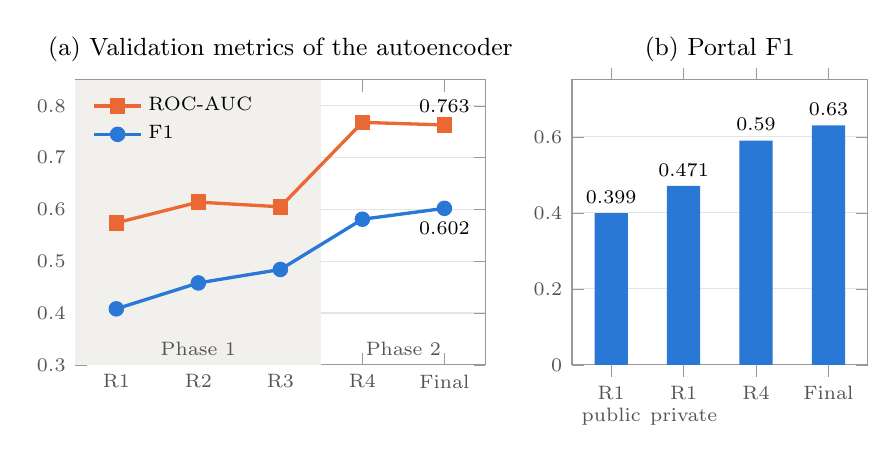
\begin{tikzpicture}
\begin{axis}[
  name=left, width=0.56\linewidth, height=5.2cm,
  ymin=0.3, ymax=0.85, xmin=0.5, xmax=5.5,
  xtick={1,2,3,4,5}, xticklabels={R1,R2,R3,R4,Final},
  ytick={0.3,0.4,0.5,0.6,0.7,0.8},
  tick label style={font=\scriptsize, text=ink2}, label style={font=\scriptsize},
  title={\small (a) Validation metrics of the autoencoder}, title style={yshift=-3pt},
  axis line style={ink2!60}, major tick style={ink2!60},
  ymajorgrids, grid style={ink2!15},
  legend style={font=\scriptsize, draw=none, fill=none, at={(0.02,0.98)}, anchor=north west},
  legend cell align=left, clip=false]
  \fill[phasebg] (axis cs:0.5,0.3) rectangle (axis cs:3.5,0.85);
  \node[font=\scriptsize, text=ink2] at (axis cs:2,0.33) {Phase 1};
  \node[font=\scriptsize, text=ink2] at (axis cs:4.5,0.33) {Phase 2};
  \addplot[sA, line width=1.2pt, mark=square*, mark size=2.2pt] coordinates {(1,0.574) (2,0.614) (3,0.605) (4,0.768) (5,0.763)};
  \addlegendentry{ROC-AUC}
  \addplot[sF, line width=1.2pt, mark=*, mark size=2.2pt] coordinates {(1,0.408) (2,0.458) (3,0.484) (4,0.581) (5,0.602)};
  \addlegendentry{F1}
  \node[font=\scriptsize, text=black, anchor=south] at (axis cs:5,0.768) {0.763};
  \node[font=\scriptsize, text=black, anchor=north] at (axis cs:5,0.595) {0.602};
\end{axis}
\begin{axis}[
  at={(left.east)}, anchor=west, xshift=1.1cm,
  width=0.44\linewidth, height=5.2cm,
  ybar, bar width=12pt, ymin=0, ymax=0.75,
  symbolic x coords={R1 pub,R1 priv,R4,Final}, xtick=data,
  xticklabels={{R1\\public},{R1\\private},R4,Final},
  xticklabel style={align=center},
  tick label style={font=\scriptsize, text=ink2},
  ytick={0,0.2,0.4,0.6},
  title={\small (b) Portal F1}, title style={yshift=-3pt},
  axis line style={ink2!60}, major tick style={ink2!60},
  ymajorgrids, grid style={ink2!15},
  point meta=explicit symbolic,
  nodes near coords, nodes near coords style={font=\scriptsize, text=black},
  enlarge x limits=0.18]
  \addplot[fill=sF, draw=none] coordinates {(R1 pub,0.399) [0.399] (R1 priv,0.471) [0.471] (R4,0.59) [0.59] (Final,0.63) [0.63]};
\end{axis}
\end{tikzpicture}
\caption{Progress across the two phases. (a) Validation F1 and ROC-AUC of the autoencoder by round; the ROC-AUC jump at R4 is the new Mahalanobis score. (b) Portal F1 of the submissions with a recorded score (R1: hybrid, public and private split; R4: Mahalanobis score; Final: autoencoder alone). R1 and R3 validation values and all portal values come from project reports.}\label{fig:progress}
\end{figure}

\begin{table}[ht]
\centering
\caption{Submissions with a recorded portal score. The Round 1 score is given as public / private split.}\label{tab:portal}
\begin{tabular}{llccc}
\toprule
Phase & Submission & Val.\ F1 & Test flagged & Portal F1 \\
\midrule
1 & Round 1 hybrid & 0.494\doc & 0.885 & 0.399 / 0.471\doc \\
2 & Round 4, Mahalanobis score & 0.581 & 0.560 & 0.59\doc \\
2 & \textbf{Final: autoencoder alone} & \textbf{0.602} & \textbf{0.622} & \textbf{0.63}\doc \\
\bottomrule
\end{tabular}
\end{table}

%======================================================================
\section{Robustness Checks on the Final Model}\label{sec:robust}
%======================================================================

In September 2026, after the final submission, we tested three possible improvements and measured how reliable the validation estimate is. All variants share one freshly trained network and one set of cached reconstruction errors, so differences reflect the variant rather than training noise. The reference row of this network scores F1 0.583, within run-to-run variation of the final model. None of the variants was adopted, and the 0.63 submission remains the final result.

\begin{table}[ht]
\centering
\caption{Robustness checks on one shared network (validation).}\label{tab:robust}
\begin{tabular}{lcccc}
\toprule
Variant & F1 & ROC-AUC & Val flag. & Test flag. \\
\midrule
Reference (final method) & 0.583 & 0.769 & 0.244 & 0.617 \\
F1-optimal threshold & 0.607 & 0.769 & 0.360 & 0.842 \\
Per-run median/MAD normalisation & 0.405 & 0.677 & 0.099 & 0.102 \\
Normal model on training windows & 0.483 & 0.611 & 0.455 & 0.833 \\
Normal model on all val.\ windows & 0.526\doc & 0.693\doc & -- & -- \\
Leave-one-run-out calibration & 0.525\doc & 0.699\doc & 0.316\doc & -- \\
\bottomrule
\end{tabular}
\end{table}

\paragraph{F1-optimal threshold.} It raised validation F1 by 0.024, within run-to-run variation, but flagged 84.2\% of test timesteps. It was not submitted.

\paragraph{Per-run normalisation.} In a diagnostic run, two validation runs scored F1 = 0 because their score peaks, although placed on the anomalies, stayed below the global threshold (Fig.~\ref{fig:timelines}). Rescaling each run by its own median and MAD was meant to fix this, but it lowered ROC-AUC from 0.769 to 0.677: it damaged the ranking itself, not only the threshold.

\paragraph{Where the normal model is fitted.} Fitting $\mu$ and $\Sigma$ on training windows lowered ROC-AUC to 0.611. Reconstruction errors on training windows are much tighter than on held-out normal windows (mean per-sensor variance 0.000144 vs 0.001727\doc), since the network was trained on them. A model fitted on all validation windows, including anomalous ones, still did better (ROC-AUC 0.693), so contamination alone does not explain the gap.

\paragraph{Validation is optimistic.} The final method fits its normal model on normal windows of the same runs it then scores, which test runs can never provide. Refitting it for each run on the other nine runs lowered ROC-AUC by 0.070 and F1 by 0.058, and ROC-AUC dropped in all ten runs. The validation figures in Section~\ref{sec:phase2} should therefore be read as optimistic estimates.

\paragraph{Validation and test scores differ.} At the final threshold, 24.1\% of validation timesteps but 62.2\% of test timesteps are flagged. If the portal computed point-wise F1, a file that flags a fraction $q$ of timesteps on a test set with prevalence $p$ would score at most $2p/(q+p)$ at perfect recall; with $q = 0.622$ and the validation prevalence $p = 0.24$ this is 0.556, below the observed 0.63. Either the test set has a higher anomaly rate, or the portal aggregates F1 differently (per run, per event or point-adjusted~\cite{kim2022towards}), or 0.63 refers to a subset of test runs. The available information does not decide between these.

\begin{figure}[ht]
\centering
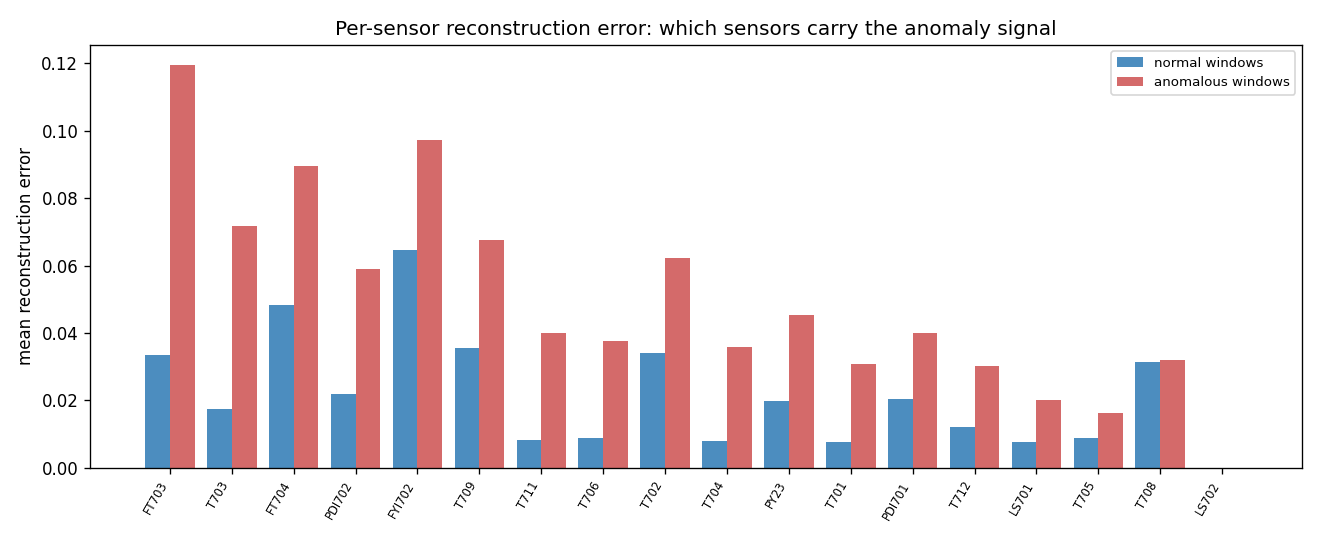
\includegraphics[width=\linewidth]{figures/per_sensor_error.png}
\caption{Mean per-sensor reconstruction error on normal and anomalous validation windows (diagnostic run of the final method). The signal concentrates in flow, pressure and temperature sensors FT703, T703, FT704, PDI702 and FYI702.}\label{fig:sensors}
\end{figure}

\begin{figure}[ht]
\centering
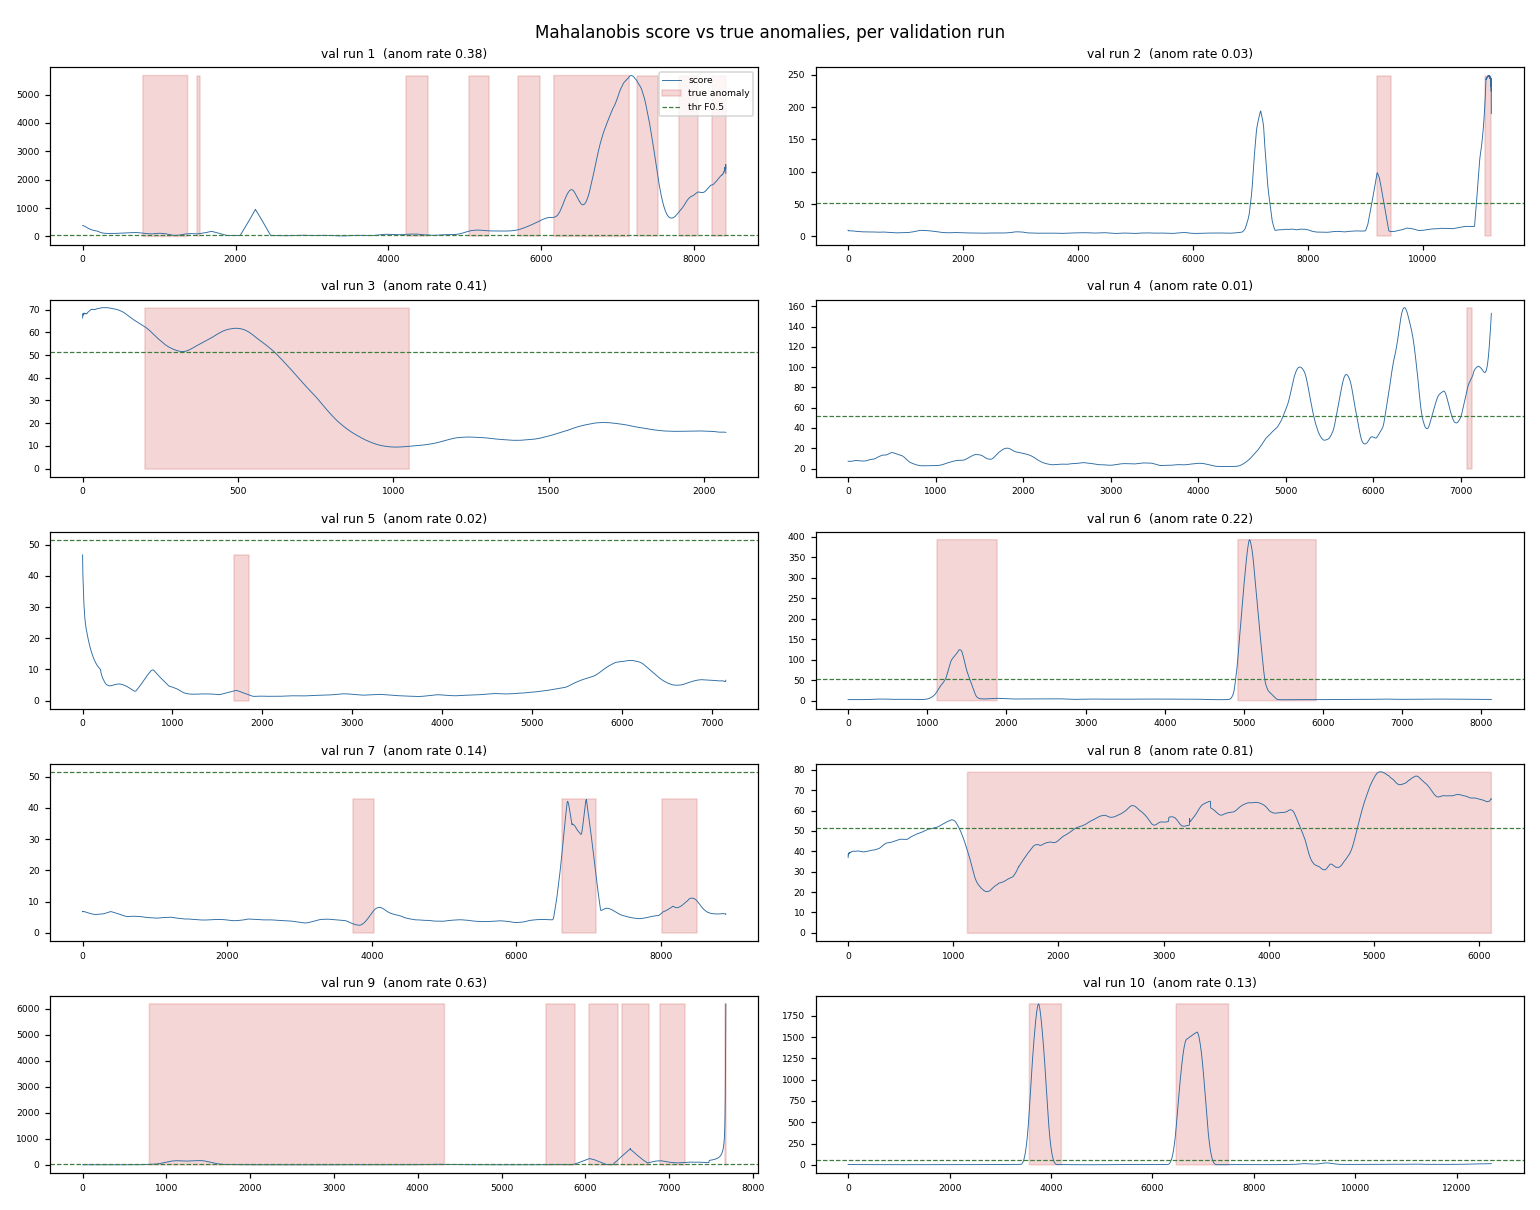
\includegraphics[width=\linewidth]{figures/val_score_timelines.png}
\caption{Anomaly score over time for the ten validation runs (diagnostic run), with labelled anomalies shaded and the global threshold drawn as a horizontal line.}\label{fig:timelines}
\end{figure}

%======================================================================
\section{Discussion}
%======================================================================

\paragraph{How Phase 2 built on Phase 1.} Phase~1 produced a pipeline whose numbers could be trusted and an architecture that sees 61 timesteps of context, but its ranking quality stayed near ROC-AUC 0.6 and its threshold over-flagged. Phase~2 kept that pipeline and architecture and changed the two weak points: the score (per-sensor Mahalanobis instead of flat error) and the threshold objective (F$_{0.5}$ instead of F1). The result was the largest gain of the project, visible both in ROC-AUC (0.605 $\rightarrow$ 0.768) and on the portal (0.471 $\rightarrow$ 0.59, then 0.63).

\paragraph{Scoring mattered more than capacity.} Checkpoint selection and the dilated architecture moved ROC-AUC very little (0.574 $\rightarrow$ 0.614 $\rightarrow$ 0.605). Changing how the model's error is scored moved it by 0.16. Figure~\ref{fig:sensors} is consistent with this: the anomaly signal sits in a few sensors, which a flat average dilutes.

\paragraph{F1 alone can mislead.} Round~3 raised F1 while ROC-AUC fell slightly, and the F1-optimal threshold in Section~\ref{sec:robust} raised F1 at identical ROC-AUC. Reporting ROC-AUC alongside F1 avoided mistaking a threshold shift for a better model.

\paragraph{Plausible ideas failed controlled tests.} Fusion, per-run normalisation and a normal model fitted on training data all had a clear motivation, and all lost when tested against the final method on the same data.

%======================================================================
\section{Limitations and Future Work}
%======================================================================

Only ten labelled runs were available, and they were used for checkpoint selection, the normal-error model, the threshold and all reported metrics, so the validation estimate is in-sample. Repeated training runs of the same configuration differ by about $\pm 0.02$ F1, and the checkpoint behind the 0.63 submission was not saved, so that exact model cannot be regenerated. The portal's F1 aggregation and the test anomaly rate are not known, which limits how far the portal score can be interpreted.

Future work should (1) use leave-one-run-out validation for every selection step, (2) establish how the portal aggregates F1 and what the test anomaly rate is before further threshold tuning, (3) address the shift between validation and test scores, (4) average scores over several training seeds to reduce run-to-run variance, and (5) save every submitted checkpoint, log and file.

%======================================================================
\section{Conclusion}
%======================================================================

We built an unsupervised detector for anomalous timesteps in 18-sensor batch-distillation data. Phase~1 established a correct pipeline and a dilated autoencoder but left ranking quality near ROC-AUC 0.6 and a portal score of 0.471. Phase~2 introduced per-sensor Mahalanobis scoring with an F$_{0.5}$ threshold, rejected fusion with LOF under run-grouped cross-validation, and produced the final model: a dilated convolutional autoencoder with portal \textbf{F1 = 0.63} (validation F1 0.602, ROC-AUC 0.763). Follow-up checks confirmed that this method could not be improved by the variants we tested and showed that its validation estimate is optimistic, which future work should correct with run-grouped validation.

\begin{credits}
\subsubsection{\ackname}
Experiments were run on the RPTU Elwetritsch cluster and on local hardware.

\subsubsection{\discintname}
The authors have no competing interests to declare that are relevant to the content of this article.
\end{credits}

\bibliographystyle{splncs04}
\bibliography{references}

\end{document}
